\chapter{Introduction}

This project aims at manipulation and visualization of DAN-Micro array data enriched by medical clinical data. The goal is to provide a tool for medical experts and micro-biologists.

\chapter{Used libraries}

\section{Java OpenGL (JOGL)}

The JOGL project hosts the development version of the Java Binding for the OpenGL API, and is designed to provide hardware-supported 3D graphics to applications written in Java (\citep{jogl:06}.

\section{Standard Widget Toolkit (SWT)}

SWT is an open source widget toolkit for Java designed to provide efficient, portable access to the user-interface facilities of the operating systems on which it is implemented (\citep{swt:06}).

\section{JGraph}

JGraph is open source graph component available for Java which uses the Swing GUI library. For more details visit \citep{jgraph:06}. 

\section{WEKA}

\begin{quotation}
Weka is a collection of machine learning algorithms for data mining tasks. The algorithms can either be applied directly to a dataset or called from your own Java code. Weka contains tools for data pre-processing, classification, regression, clustering, association rules, and visualization. It is also well-suited for developing new machine learning schemes (\citep{weka:06}).
\end{quotation}

\chapter{Class Design}

\section{Modules}

The Cerberus Software can be devided in several module packages.
The packages itself are intended to be as seperate as possible with a clear interface for moudle inter-communication. 
The simple reason for this approach is the easier changeability and extendability.
In \stdref{gfx:cerberus_module_design} the module design is visualized using an UML package diagram.

\begin{figure}[ht]
\centering
\scalebox{0.6}{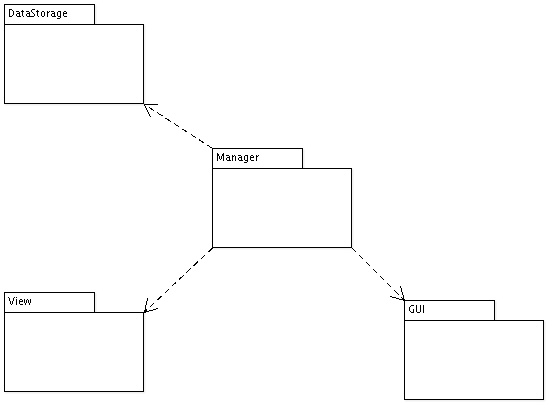
\includegraphics{gfx/CerberusModuleDesign}} 
\caption[Cerberus Module Design]{\textit{Cerberus Modules}} 
\label{gfx:cerberus_module_design}
\end{figure}

In the following sections the modules are explained in more detail.

\section{Manager Module}

All components are handled by Mangers. This opens the possibility to use Abstract Factories (Design Pattern "Abstract  Factory"). Since all above described components are only Interfaces, all components / objects can be created by factories (Design Pattern "Factory").

\section{Data Module}

\subsection{Internal Data Management}

\minisec{DataStorage}
Arrays filled with INT, FLOAT, DOUBLE, STRING, BOOLEAN

\minisec{Selection}
Define regions on DataStorage-Objects

\minisec{Set}
Holds a collection of Selections which refer to a DataStorage.
Pipe-and-Filers Design Pattern (DataStorage-Selection-Set)
Selection and Set can be accessed by Iterators. Design Pattern "Iterator".

\begin{figure}[ht]
\centering
\scalebox{0.6}{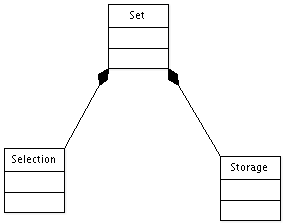
\includegraphics{gfx/DataModuleClassDesign}} 
\caption[Data Module Class Design]{\textit{Data Module Class Design}} 
\label{gfx:data_module_class_design}
\end{figure}

\subsection{External Data}

\minisec{Micro-Array Data file}

\begin{itemize}
\item \textbf{Description: } One file stores one micro-array experiment containing all Genes/Proteins.
\item \textbf{Extension:}  *.grp
\item \textbf{File size: } ~ 8 MB
\item \textbf{Dimension: } [38000 Genes] x [1 probe] x [ ~10 values + (15 derived statistical values) ]
\item \textbf{Format: } ASCII, header, table of values
\end{itemize}

\minisec{Clinical Excel files}

\begin{itemize}
\item \textbf{Description: } Each row represents one patient; each column contains data on the patient.
\item \textbf{Extension: } *.xls  and  *.csv
\item \textbf{File size: } > 1 MB
\item \textbf{Dimension: } [~40 medical parameters] x [ 2000 patients]
\item \textbf{Format: } EXCEL-file, Header row, table of values
\end{itemize}

\minisec{Pathway data file}

\begin{itemize}
\item \textbf{Description: } Biological and medical pathways. For details see \fullref{msec:pathway_description}.
\item \textbf{Extension: } *.xml
\item \textbf{File size: } each < 1 MB
\item \textbf{Dimension: } [~3000] x [ directed cyclic graph]
\item \textbf{Format: } XML-file
\end{itemize}

\section{GUI Module}

The application will be built using the SWT. 
The Frame class is the basis of all GUI elements in the Cerberus application.
The inheritence structure is shown in \stdref{gfx:gui_module_class_design} 
This class is implemented as an interface which makes it basically possible to exchange the GUI library SWT with Swing.
The Swing dependency is needed anyway because JGraph is used for visualizing and editing Graphs (needed for Pathways).
JGraph takes only an Swing Frame for drawing. Therefore the Swing Frame needs to be embedded in a SWT Frame.
Obviously this is a workaround but JGraph is a very powerful Graph Library on which we don't want to surrender.
The Jogl render area can be embedded in an SWT Fram without problems.

\begin{figure}[ht]
\centering
\scalebox{0.7}{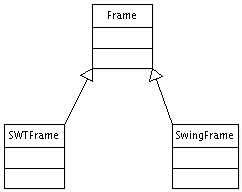
\includegraphics{gfx/GUIModuleClassDesign}} 
\caption[GUI Module Class Design]{\textit{GUI Module Class Design}} 
\label{gfx:gui_module_class_design}
\end{figure}

\section{View Module}

In \stdref{gfx:view_module_class_design} the class design of the view module is visualized in UML.
All special view types (e.g. heatmaps, pathways, etc.) are inherited from a general View interface.
The abstract interface hides the implementation of the specific Views.
The Views are created by a ViewFactory (which follows the Abstract Factory Design Pattern).

\begin{figure}[ht]
\centering
\scalebox{0.6}{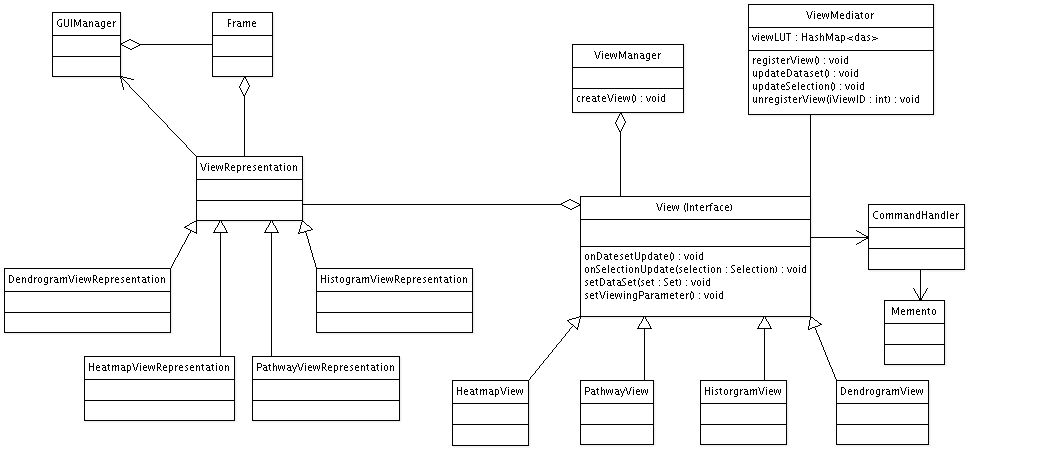
\includegraphics{gfx/ViewModuleClassDesign}} 
\caption[View Module Class Design]{\textit{View Module Class Design}} 
\label{gfx:view_module_class_design}
\end{figure}

\minisec{DataViewMediator}
The View objects are stored in a HashMap in the ViewMediator. The key in the Map is the Set ID of the Dataset and the value the View Object. The map can then be used as a lookup table for finding out the relations among the View objects. Generally (in most cases) a View influences another View only if they operate on the same Set of data. 
The ViewMediator follows the well known Mediator Design Pattern, where several Objects can communicate over a common module.
Therefore the usage of the Mediator Pattern eliminates the need of Objects to refer to each other directly which reduces the implementation effort. Also in case of a new View type it has to only registered in the ViewMediator without knowing an referring to the other Views. In the Mediator class special update methods are implemented, which are called when in a View some kind of event occurs. The View calls on of these update models (as the case may be) and the update method in the Mediator finds out all related Views and triggers the update. The update method in the view knows then how to react on that update. For example a Heatmap has to visualize an selection completely different as an Dendrogram.

The ViewMediator reacts on two basic events.
\begin{itemize}
\item \textbf{selectionUpdate: } The selection update is triggered when the user selects a portion or a region of a View, which influences other dependent Views.
\item \textbf{dataSetUpdate: } The dataSetUpdate is called when the Set of data changes in a View. For example when a clustering algorithm is performed on the Set of data which results in an update of all Views, which visualize these 
\end{itemize}

\subsection{Heatmap View}

\subsection{Dendrogram View}

\minisec{Description}
A Dendrogram is a tree diagram that is mostly used to show the result of clustering alogrithms.

\subsection{Pathway View}

\minisec{Description}
\label{msec:pathway_description}

Collection of Proteins, that interact with each other and thus occur co-regulated or counter-regulated in the micro-array data-sets. A pathway is a directed cyclic graph consisting of Proteins, which can be traversed in forward or backward order. One Protein may occur several times in different nodes. The edges of the graph can be tagged with additional information. For instance required or produced biochemical energy (ADP +Pi  <==> ATP) or (NADP <==> NADPH). Some pathways are irreversible and thus only traverse in one direction, like "Glukose-Spalltung = Glykolyse". Once this kind of pathway is triggered it is "executed". Other Pathways like "Umbau von Zucker" or the Fat-Cycle can be traversed back and forth.

\begin{figure}[ht]
\centering
\scalebox{0.5}{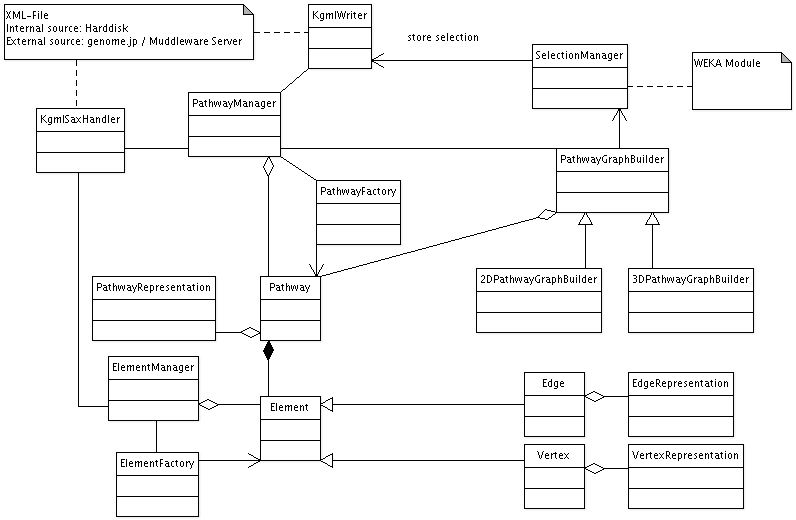
\includegraphics{gfx/PathwayClassDesign}} 
\caption[Pathway Class Design]{\textit{Pathway Class Design}} 
\label{gfx:pathway_class_design}
\end{figure}

\subsection{Histogram View}

\subsection{Combination and interaction of Views}




